%=============================================================================
%  CSE 465 Project Report -- North South University
%  Reasoning Termination, Not Reasoning Capability
%  Compile in Overleaf with pdfLaTeX. Run twice for the ToC/refs.
%=============================================================================
\documentclass[12pt,a4paper,oneside]{report}

\usepackage[T1]{fontenc}
\usepackage[utf8]{inputenc}
\usepackage{newtxtext,newtxmath}     % Times New Roman
\usepackage[margin=1in]{geometry}
\usepackage{setspace}
\usepackage{graphicx}
\usepackage{booktabs}
\usepackage{amsmath}
% newtxmath already defines \Bbbk; free the name before amssymb redefines it
\let\Bbbk\relax
\usepackage{amssymb}
\usepackage{caption}
\usepackage{array}
\usepackage{multirow}
\usepackage{enumitem}
\usepackage{tikz}
\usepackage{xcolor}
\usepackage[hidelinks]{hyperref}
\usepackage{titlesec}
\usepackage{tocloft}
\usetikzlibrary{shapes.geometric,arrows.meta,positioning,calc}

\onehalfspacing
\setlength{\parindent}{0pt}
\setlength{\parskip}{6pt}

% chapter headings in template style
\titleformat{\chapter}[hang]{\normalfont\Large\bfseries}{\thechapter}{1em}{}
\titlespacing*{\chapter}{0pt}{0pt}{20pt}

\captionsetup[figure]{font=small,labelfont=bf}
\captionsetup[table]{font=small,labelfont=bf}

\definecolor{nsublue}{RGB}{31,56,100}

% ---- shorthand -------------------------------------------------------------
\newcommand{\boxedans}{\texttt{\textbackslash boxed\{\}}}
\newcommand{\vt}{VibeThinker-3B}

\begin{document}

%=============================================================================
% COVER PAGE
%=============================================================================
\begin{titlepage}
\centering
\vspace*{0.5cm}

{\large\bfseries Department of Electrical and Computer Engineering}\\[4pt]
{\large\bfseries North South University}\\[30pt]

{\large CSE 465 --- Course Project}\\[40pt]

{\LARGE\bfseries\color{nsublue}
Reasoning Termination, Not Reasoning Capability,\\[6pt]
Bounds Small Language Model Performance\\[6pt]
on Competition Mathematics\par}

\vspace{12pt}
{\large\itshape A Budget-Forcing Study of VibeThinker-3B on AIME 2025\par}

\vspace{50pt}

{\large\bfseries Abu Ahmad \quad ID\# 2121725042}\\[60pt]

{\large\bfseries Faculty Advisor:}\\[8pt]
{\large Dr. Nabeel Mohammed [NbM]}\\[4pt]
{\large Professor}\\[4pt]
{\large ECE Department}\\[30pt]

{\large Summer, 2026}

\vfill
\end{titlepage}

%=============================================================================
% APPROVAL
%=============================================================================
\chapter*{APPROVAL}
\addcontentsline{toc}{chapter}{APPROVAL}

Abu Ahmad (ID \# 2121725042) from the Electrical and Computer Engineering
Department of North South University has worked on the CSE 465 project titled
``Reasoning Termination, Not Reasoning Capability, Bounds Small Language Model
Performance on Competition Mathematics'' under the supervision of
\textbf{Dr.\ Nabeel Mohammed} in partial fulfillment of the requirement for the
degree of Bachelor of Science in Engineering, and it has been accepted as
satisfactory.

\vspace{40pt}
\textbf{Supervisor's Signature}

\vspace{25pt}
\dotfill

Dr.\ Nabeel Mohammed\\
Professor\\
Department of Electrical and Computer Engineering\\
North South University\\
Dhaka, Bangladesh.

\vspace{35pt}
\textbf{Chairman's Signature}

\vspace{25pt}
\dotfill

Dr.\ Rajesh Palit\\
Professor and Chairman\\
Department of Electrical and Computer Engineering\\
North South University\\
Dhaka, Bangladesh.

%=============================================================================
% DECLARATION
%=============================================================================
\chapter*{DECLARATION}
\addcontentsline{toc}{chapter}{DECLARATION}

This is to declare that this project is my original work. No part of this work
has been submitted elsewhere partially or fully for the award of any other
degree or diploma. All project-related information will remain confidential and
shall not be disclosed without the formal consent of the project supervisor.
Relevant previous works presented in this report have been properly
acknowledged and cited. The plagiarism policy, as stated by the supervisor, has
been maintained.

All numerical results reported in Chapter~4 were measured by the author on the
stated hardware. No result in this report is estimated, projected, or carried
over from the source publications. Where a quantity was not measured, it is
explicitly labelled as such.

\vspace{50pt}
\textbf{Student's name \& Signature}

\vspace{35pt}
1. Abu Ahmad

\vspace{10pt}
\rule{7cm}{0.4pt}

%=============================================================================
% ACKNOWLEDGEMENTS
%=============================================================================
\chapter*{ACKNOWLEDGEMENTS}
\addcontentsline{toc}{chapter}{ACKNOWLEDGEMENTS}

The author would like to express heartfelt gratitude towards the project and
research supervisor, \textbf{Dr.\ Nabeel Mohammed}, Professor, Department of
Electrical and Computer Engineering, North South University, Bangladesh, for
his invaluable support, precise guidance, and advice pertaining to the
experiments, research, and theoretical studies carried out during the course of
the current project, and also in the preparation of this report.

Furthermore, the author would like to thank the Department of Electrical and
Computer Engineering, North South University, Bangladesh, for facilitating this
research. Acknowledgement is also due to Weibo AI for openly releasing the
VibeThinker-3B model weights, to the vLLM project for the inference engine that
made this study feasible on free-tier hardware, and to Kaggle for providing the
GPU allocation on which all experiments were run.

Finally, the author would like to thank his loved ones for their countless
sacrifices and continual support.

%=============================================================================
% ABSTRACT
%=============================================================================
\chapter*{ABSTRACT}
\addcontentsline{toc}{chapter}{ABSTRACT}

\begin{center}
\textbf{Reasoning Termination, Not Reasoning Capability, Bounds Small Language
Model Performance on Competition Mathematics}
\end{center}

Compact language models have recently begun to match the performance of far
larger systems on verifiable reasoning tasks, but their reported accuracy is
routinely measured under generous generation limits that ordinary deployments
cannot afford. This project asks a narrower and more practical question: when a
small reasoning model fails on a competition mathematics problem, has it failed
to solve the problem, or has it merely failed to stop and state the answer it
already possesses. A three-billion-parameter reasoning model was evaluated
without any modification to its weights on thirty problems from a recent
national mathematics olympiad, sampled four times each, across generation
budgets spanning one thousand to thirty-two thousand tokens. The results
separate the two failure modes cleanly. Among the samples that terminated
naturally, virtually every one produced the correct answer, whereas almost every
sample that exhausted its budget scored zero, not because its reasoning was
wrong but because no answer had yet been written down. The entire shortfall
between the published accuracy and the reproduced accuracy is therefore
attributable to truncation rather than to reasoning error. A lightweight
intervention that interrupts the model at its budget limit and compels it to
commit to an answer was then evaluated. The intervention improved accuracy
significantly at every budget tested, never converted a correct answer into an
incorrect one across one hundred and thirty-nine interventions, and proved
insensitive to the wording used to trigger it, with an elaborate two-stage
variant costing more than twice the computation for no measurable benefit. A
single intervened sample outperformed the best of four unintervened samples at
the smaller budgets, establishing that the method exceeds the theoretical
ceiling of any technique that merely selects among existing candidate answers.
Analysis of the recoverable population shows the intervention captures
approximately four fifths of the answers latent in truncated traces, indicating
that the remaining headroom lies in generating reasoning rather than in
extracting it. All experiments were completed within twenty-three graphics
processing unit hours on freely available hardware.

%=============================================================================
% FRONT MATTER LISTS
%=============================================================================
\tableofcontents
\listoffigures
\listoftables
\clearpage

%=============================================================================
% CHAPTER 1
%=============================================================================
\chapter{Introduction}

\section{Background and Motivation}

Large language models have improved dramatically at multi-step logical reasoning
over the past two years, driven largely by the introduction of reinforcement
learning with verifiable rewards into the post-training stage
\cite{deepseekr1,deepseekmath}. Under this paradigm a model is rewarded only
when its final answer can be mechanically checked, which allows it to discover
effective intermediate reasoning strategies without any step-level human
supervision. The resulting systems produce long chains of thought, often
spanning tens of thousands of tokens, before committing to a final answer.

Until recently, frontier performance on demanding verifiable benchmarks was
concentrated in models with hundreds of billions of parameters. VibeThinker-3B
\cite{vibethinker} challenged this assumption. Built on a three-billion-parameter
dense backbone \cite{qwen25coder} and post-trained through curriculum supervised
fine-tuning, multi-domain reinforcement learning, offline self-distillation, and
instruction alignment, it reports 91.4 on AIME 2025 and 94.3 on AIME 2026,
placing it within the performance band of systems two orders of magnitude
larger. Its authors advance the \emph{Parametric Compression--Coverage
Hypothesis}: verifiable reasoning compresses into a compact reusable core,
whereas open-domain knowledge requires broad parameter coverage and does not.

This result matters practically as well as scientifically. A three-billion-
parameter model can be served on a single consumer graphics card, which places
frontier-level mathematical reasoning within reach of individual researchers,
students, and institutions in resource-constrained settings. The
democratisation argument, however, carries a hidden assumption that this project
set out to examine.

Reported benchmark scores for reasoning models are obtained under generous
generation limits. The VibeThinker-3B documentation recommends a maximum
generation length of $40{,}960$ tokens. Generating forty thousand tokens for a
single problem is expensive: on the class of hardware available to a student, it
takes minutes per sample, and the cost compounds when multiple samples are drawn
per problem, as every serious evaluation protocol requires. A model whose
frontier accuracy is only reachable at forty thousand tokens per sample is far
less accessible than its parameter count suggests.

This gives rise to the question that motivates the present work. When such a
model is given a smaller budget and its accuracy falls, \emph{what exactly has
been lost}. There are two candidate explanations with sharply different
consequences:

\begin{enumerate}
\item \textbf{Capability loss.} The model requires the full reasoning trace to
reach the answer. A shorter budget genuinely prevents the derivation, and
accuracy is irrecoverable without spending the tokens.
\item \textbf{Termination failure.} The model reaches the answer earlier but
continues verifying, exploring alternatives, and re-deriving. The budget expires
mid-deliberation and the trace is discarded, not because it is wrong, but
because no answer was ever written down.
\end{enumerate}

Under the first explanation nothing can be done cheaply. Under the second, the
loss is an artifact of the evaluation protocol rather than a property of the
model, and a very inexpensive intervention should recover much of it. The two
explanations are empirically distinguishable, and distinguishing them is the
central contribution of this project.

\section{Purpose and Goal of the Project}

The purpose of this project is to determine which of the two failure modes above
accounts for the accuracy loss of a compact reasoning model under a constrained
generation budget, and to evaluate whether the loss can be recovered without
retraining the model.

Three constraints shaped the scope. First, no model weights were to be modified;
the study is inference-time only. Second, all computation had to fit within the
free tier of a public cloud notebook platform, capping the budget at thirty
graphics processing unit hours per week on a single Tesla T4. Third, every
reported number had to be measured on that hardware rather than carried over
from a publication.

The contributions of this report are as follows.

\begin{itemize}
\item \textbf{A diagnosis separating termination failure from capability
failure.} Per-problem analysis shows that the count of correct samples equals
the count of naturally terminated samples almost exactly. Among the 95 of 120
samples that terminated naturally, essentially all were correct; of the 25 that
were truncated, 23 scored zero for want of a parseable answer. The entire
$91.4 \rightarrow 80.8$ shortfall is therefore a truncation artifact. To the
author's knowledge this decomposition has not previously been reported for a
model in this size class.

\item \textbf{A measurement of budget forcing on a compact reasoning model.}
Budget forcing \cite{s1} was evaluated at four generation budgets. It yields
statistically significant gains at every budget, confirmed by McNemar's test for
paired proportions, and is shown to be \emph{strictly non-destructive}: across
139 interventions, not one correct answer was converted into an incorrect one.

\item \textbf{A negative result on prompt engineering for budget forcing.} Three
intervention phrasings, including a two-stage summarise-then-answer variant,
were compared. They are statistically indistinguishable, while the two-stage
variant costs $2.1\times$ more computation. What matters is that the model is
compelled to commit at all, not how it is asked.

\item \textbf{An upper-bound analysis establishing that budget forcing exceeds
the selection ceiling.} A single intervened sample outperforms the best of four
unintervened samples at the smaller budgets. Since $\text{pass}@k$ bounds any
method that \emph{selects} among existing samples, this quantifies why
selection-based test-time methods are the wrong tool in this regime.
Restricting to the recoverable population, the intervention captures
approximately 80\% of the answers latent in truncated traces, indicating that
the remaining headroom lies in generation rather than extraction.
\end{itemize}

A methodological contribution supports the above. Because autoregressive
generation is prefix-consistent, the first $N$ tokens of a longer generation are
distributionally identical to a budget-$N$ generation. Storing traces at the
largest budget therefore permits every smaller budget to be scored on a central
processing unit at zero additional cost. This was validated empirically and
reduced the compute required for the budget sweep by roughly a factor of three.

\section{Organization of the Report}

Chapter 2 reviews the relevant literature on compact reasoning models,
inference-time scaling, and selection-based test-time methods, and identifies
the gap this project addresses. Chapter 3 presents the methodology, comprising
the system design, the software and hardware components, and the implementation
of the evaluation harness and the budget-forcing intervention. Chapter 4
reports the experiments, results, statistical analysis, and discussion,
including the mechanism by which the intervention succeeds and fails. Chapter 5
concludes with a summary, an explicit statement of limitations, and directions
for future improvement.

%=============================================================================
% CHAPTER 2
%=============================================================================
\chapter{Research Literature Review}

\section{Existing Research and Limitations}

\subsection*{Reinforcement learning for verifiable reasoning}

Guo et al.\ \cite{deepseekr1} demonstrated with DeepSeek-R1 that rule-based
reinforcement learning over verifiable rewards, built on the group-relative
policy optimisation objective introduced in DeepSeekMath \cite{deepseekmath},
elicits sophisticated long-horizon reasoning without step-level supervision. The
model is rewarded solely on final-answer correctness and output format, and
learns intermediate reasoning strategies on its own. This established the
training recipe that virtually all subsequent reasoning models, including the
one studied here, follow.

Xu et al.\ \cite{vibethinker} applied this paradigm in the strictly small-model
regime, producing VibeThinker-3B. Their pipeline comprises curriculum two-stage
supervised fine-tuning, multi-domain reinforcement learning under a single
64K-token context window, an efficiency-oriented Long2Short stage, offline
self-distillation, and instruction-oriented alignment. The model reports 91.4 on
AIME 2025, 94.3 on AIME 2026, and 80.2 Pass@1 on LiveCodeBench v6. Two aspects
of that work bear directly on this project. First, the reported evaluation
protocol imposes no output length cap beyond the model's maximum generation
length, so the published figures represent performance under an effectively
unconstrained budget. Second, the authors note that the model's weakness lies in
knowledge-intensive tasks rather than in reasoning procedure. Neither the paper
nor its accompanying documentation reports how accuracy degrades when the
generation budget is constrained, which is precisely the regime a deployment on
modest hardware occupies.

\subsection*{Inference-time scaling}

A parallel line of work improves accuracy at inference time without touching
model weights. Wang et al.\ \cite{selfconsistency} introduced self-consistency,
which samples multiple reasoning chains and returns the majority answer.
Madaan et al.\ \cite{selfrefine} proposed self-refinement, in which a model
critiques and revises its own output iteratively. Xu et al.\ \cite{vibethinker}
describe Claim-Level Reliability Assessment, which extracts decision-relevant
claims from each sampled trajectory, has the model verify them, and aggregates
candidate answers weighted by a nonlinear reliability score, reporting an
improvement from 94.3 to 97.1 on AIME 2026 at $K=32$ samples.

These methods share a structural property that turns out to be decisive. All
three operate by \emph{selecting or refining among candidate answers that
already exist}. Their achievable accuracy is therefore bounded above by
$\text{pass}@k$, the fraction of problems for which at least one of the $k$
sampled trajectories is correct. When sampled trajectories agree with one
another, or when they produce no answer at all, these methods have nothing to
act upon. Section~4.6 shows this bound is binding in the present setting.

\subsection*{Budget forcing}

Muennighoff et al.\ \cite{s1} introduced budget forcing as a component of the s1
test-time scaling recipe. When a model reaches a prescribed token budget, the
decoding procedure appends a phrase that terminates the reasoning segment and
demands a final answer, forcing commitment rather than allowing the generation to
be discarded. Their work applies the technique primarily as a mechanism for
\emph{extending} reasoning, in combination with supervised fine-tuning on a
curated reasoning corpus. Its use as a standalone recovery mechanism on a frozen
model, and its interaction with the accuracy-versus-budget curve, are not
characterised.

\subsection*{Identified limitations and the resulting gap}

A detailed examination of the literature yields the following observations.
\begin{enumerate}[label=(\roman*)]
\item Published accuracies for compact reasoning models are reported under
effectively unconstrained generation budgets, and the degradation curve under
realistic budgets is not characterised, despite deployment cost being the
principal argument for compact models.
\item Failure analyses report aggregate accuracy without separating incorrect
answers from \emph{absent} answers. A truncated trace and an erroneous trace are
scored identically at zero, which conflates two failure modes with entirely
different remedies.
\item Test-time scaling methods are evaluated in regimes where sampled
trajectories disagree, so their applicability where trajectories agree, or
produce nothing, is untested.
\item Budget forcing has been evaluated as an extension mechanism accompanied by
fine-tuning, but not as a standalone recovery mechanism on a frozen model, and
no measurement exists of whether it can \emph{damage} an otherwise correct
output.
\end{enumerate}

These observations motivate the present project, which characterises the
accuracy-versus-budget curve for a compact reasoning model, decomposes its
failures into truncation and error, evaluates budget forcing as a standalone
recovery mechanism with an explicit test for harm, and bounds the achievable
recovery against both the selection ceiling and the extraction ceiling.

%=============================================================================
% CHAPTER 3
%=============================================================================
\chapter{Methodology}

\section{System Design}

\subsection{Problem formulation}

Let $\pi$ denote the frozen policy of the language model and $q$ a problem
statement. Under an unconstrained budget the model emits a token sequence
$y = (y_1,\dots,y_T)$ terminating in an end-of-sequence token, from which a
final answer $a(y)$ is extracted by parsing the last \boxedans{} expression.
Under a budget $B$ the generation is truncated at $\min(T,B)$ tokens.

Define the termination indicator
\begin{equation}
\tau_B(y) \;=\;
\begin{cases}
1, & T \le B \quad \text{(terminated naturally)}\\[2pt]
0, & T > B \quad \text{(truncated)}
\end{cases}
\label{eq:tau}
\end{equation}

and the correctness indicator $c_B(y) = \mathbb{1}\!\left[a(y_{1:\min(T,B)}) =
a^{\star}\right]$ where $a^{\star}$ is the ground-truth answer. The two
competing hypotheses stated in Section 1.1 make different predictions about the
joint distribution of $\tau_B$ and $c_B$. Under the capability hypothesis,
truncated traces are wrong because their reasoning is incomplete, so correctness
should degrade smoothly with $B$ among terminated and truncated samples alike.
Under the termination hypothesis, correctness should be near-total among
terminated samples and near-zero among truncated ones, giving
\begin{equation}
\Pr\!\left[c_B = 1 \mid \tau_B = 1\right] \;\approx\; 1,
\qquad
\Pr\!\left[c_B = 1 \mid \tau_B = 0\right] \;\approx\; 0 .
\label{eq:hypotheses}
\end{equation}

\subsection{Budget forcing}

Budget forcing intervenes on truncated samples only. Given a truncated prefix
$y_{1:B}$ and a fixed forcing phrase $\phi$, the model is invoked a second time
on the concatenation and decoded greedily for a short continuation:
\begin{equation}
\hat{a} \;=\; a\!\left(\,\pi\!\left(q \oplus y_{1:B} \oplus \phi\right)\,\right),
\qquad
\phi = \texttt{"</think> ... the final answer is \textbackslash boxed\{"} .
\label{eq:forcing}
\end{equation}
Samples that terminated naturally are left untouched. The procedure adds no
trainable parameters and generates on the order of five tokens per intervened
sample.

Three phrasings of $\phi$ were compared: a bare demand ($V_1$), a soft-deadline
formulation ($V_3$), and a two-stage variant ($V_2$) in which the model first
produces a structured summary of its established results and only then is asked
for the answer.

\subsection{Prefix consistency and free budget derivation}

Because generation is autoregressive, the conditional distribution of the first
$N$ tokens does not depend on the budget at which generation was stopped.
Consequently, for $N \le B$,
\begin{equation}
y_{1:N} \sim \pi(\cdot \mid q) \Big|_{\text{budget } N}
\quad\text{is distributionally identical to}\quad
\left(y \sim \pi(\cdot \mid q)\Big|_{\text{budget } B}\right)_{1:N}.
\label{eq:prefix}
\end{equation}
Storing full traces at the largest budget therefore permits every smaller budget
to be scored on a CPU at zero GPU cost. This identity was validated empirically
(Section 4.2) and is the reason the budget sweep in this project was affordable.

\subsection{Overall pipeline}

Figure~\ref{fig:pipeline} summarises the experimental design.

\begin{figure}[htbp]
\centering
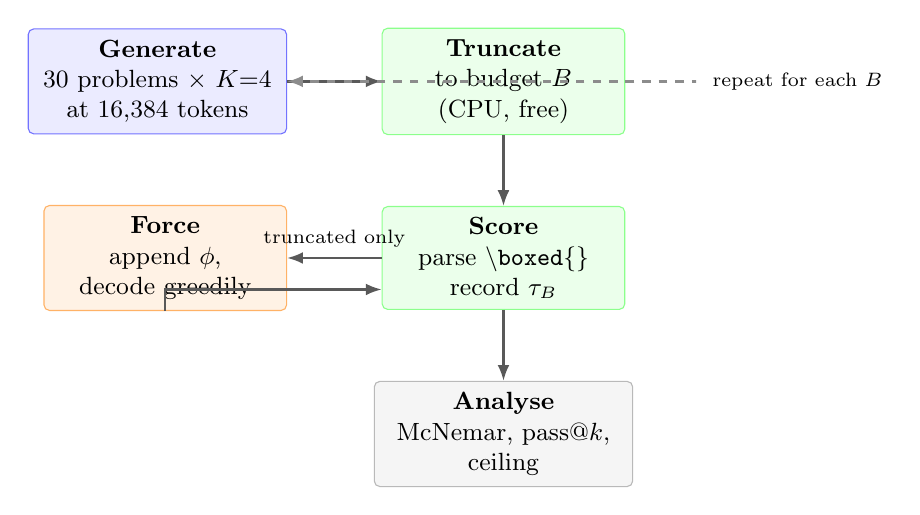
\begin{tikzpicture}[
  node distance=8mm,
  box/.style={draw,rounded corners=2pt,align=center,minimum height=11mm,
              inner sep=4pt,font=\small},
  gen/.style={box,fill=blue!8,draw=blue!55,text width=30mm},
  cpu/.style={box,fill=green!8,draw=green!45,text width=28mm},
  gpu/.style={box,fill=orange!10,draw=orange!60,text width=28mm},
  ana/.style={box,fill=gray!8,draw=gray!55,text width=30mm},
  ar/.style={-{Latex[length=2mm]},thick,draw=black!65}
]
\node[gen] (gen) {\textbf{Generate}\\30 problems $\times$ $K{=}4$\\at 16{,}384 tokens};
\node[cpu, right=12mm of gen] (trunc) {\textbf{Truncate}\\to budget $B$\\(CPU, free)};
\node[cpu, below=9mm of trunc] (score) {\textbf{Score}\\parse \boxedans{}\\record $\tau_B$};
\node[gpu, left=12mm of score] (force) {\textbf{Force}\\append $\phi$,\\decode greedily};
\node[ana, below=9mm of score] (stats) {\textbf{Analyse}\\McNemar, $\text{pass}@k$,\\ceiling};

\draw[ar] (gen) -- (trunc);
\draw[ar] (trunc) -- (score);
\draw[ar] (score) -- node[above,font=\scriptsize]{truncated only} (force);
\draw[ar] (force) |- ($(score.west)+(0,-4mm)$);
\draw[ar] (score) -- (stats);
\draw[ar,dashed,draw=black!45] (trunc.east) -- ++(9mm,0) |- node[right,font=\scriptsize,pos=0.25]{\;repeat for each $B$} (gen.east);
\end{tikzpicture}
\caption[Experimental pipeline]{Experimental pipeline. Generation is performed
once at the largest budget. Every smaller budget is obtained by truncating the
stored traces on a CPU, which costs nothing; only the forcing step returns to
the GPU, and it acts on truncated samples alone.}
\label{fig:pipeline}
\end{figure}

\section{Hardware and Software Components}

\subsection{Model and dataset}

The subject model is \texttt{WeiboAI/VibeThinker-3B} \cite{vibethinker}, a
three-billion-parameter dense decoder. Its weights were \emph{never modified};
every experiment is inference-only.

The benchmark is the 30-problem AIME 2025 set, obtained from the public
\texttt{math-ai/aime25} release. AIME 2026 was used in the original publication
but is not available as a public dataset, so AIME 2025 was substituted. This
substitution is advantageous: \cite{vibethinker} reports 91.4 for AIME 2025,
providing a published reference against which the evaluation harness could be
validated. Answers are integers in $[0,999]$, which permits exact matching and
removes any need for a judge model.

\subsection{Inference engine}

Initial measurements used the HuggingFace \texttt{transformers} generation loop
and achieved 15.2 tokens per second, which projected to over one hundred GPU
hours for the planned sweep and was therefore infeasible. The engine was
replaced with vLLM \cite{vllm}, whose continuous batching and prefix sharing
raised throughput to 246.4 tokens per second at $K=32$, a $16.2\times$
improvement. Table~\ref{tab:tools} lists the components.

\begin{table}[htbp]
\centering
\caption{Software and hardware components}
\label{tab:tools}
\small
\newcolumntype{L}[1]{>{\raggedright\arraybackslash}p{#1}}
\begin{tabular}{@{}L{2.3cm}L{3.5cm}L{3.0cm}L{5.6cm}@{}}
\toprule
\textbf{Tool} & \textbf{Function} & \textbf{Alternatives} & \textbf{Why selected} \\
\midrule
vLLM 0.26.0 & Inference engine & HF \texttt{transformers}, TensorRT-LLM &
$16.2\times$ faster via continuous batching and prefix sharing; the workload is
many samples from one prompt, its best case \\
\addlinespace
Tesla T4 (16\,GB) & Accelerator & A100, TPU v4 & Only hardware available on the
free tier; imposes \texttt{float16} and rules out FlashAttention-2 \\
\addlinespace
VibeThinker-3B & Subject model & Qwen3-4B, Phi-4-mini & Frontier accuracy at 3B;
published AIME 2025 score permits harness validation \\
\addlinespace
\texttt{math-ai/} \texttt{aime25} & Benchmark & AIME 2024, HMMT & Integer answers
allow exact matching; matches a published reference number \\
\addlinespace
Kaggle Notebooks & Compute platform & Colab, Lambda Labs & 30 GPU-hours per week
at no cost; batch execution survives disconnection \\
\bottomrule
\end{tabular}
\end{table}

\subsection{Hardware constraints and their consequences}

The Tesla T4 uses the Turing architecture (compute capability 7.5), which has
three consequences that shaped the implementation. FlashAttention-2 requires
compute capability 8.0 or above, so vLLM falls back to a Triton attention
backend. \texttt{bfloat16} is unsupported, making \texttt{float16} mandatory.
Most importantly, the key-value cache holds $192{,}272$ tokens at 90\% memory
utilisation, so the number of concurrently decodable sequences is
\begin{equation}
\text{concurrency} \;=\; \frac{192{,}272}{\texttt{max\_model\_len}} .
\label{eq:concurrency}
\end{equation}
Throughput is roughly proportional to concurrency, which is why a 32K context
sustained only 60--71 tokens per second while an 8K context sustained 246.

\section{Software Implementation}

\subsection{Evaluation harness}

Decoding parameters were frozen across every experimental arm: temperature
$1.0$, $\text{top-}p = 0.95$, seed $0$, and $K=4$ samples per problem. The
prompt is produced by the model's own chat template with no additional
instruction. Answer extraction locates the final \boxedans{} expression with a
brace-depth parser, then extracts the first integer. A single implementation is
shared by all arms so that a change cannot silently apply to one condition only.

\subsection{Termination logging}

The decisive measurement of this project requires distinguishing a wrong answer
from an absent one. For every sample the harness records the completion reason
reported by the engine, the token length, whether a \boxedans{} expression was
parseable, and the extracted value. Aggregate accuracy alone cannot support the
central claim; the per-sample termination reason is what makes
Equation~\eqref{eq:hypotheses} testable.

\subsection{Statistical procedure}

Budget forcing operates on the same samples before and after intervention, so
the design is \emph{paired} and an unpaired test would be inappropriate.
McNemar's test with continuity correction is used throughout. With $b$ denoting
samples that changed from incorrect to correct and $c$ those that changed from
correct to incorrect,
\begin{equation}
\chi^{2} \;=\; \frac{\left(|b - c| - 1\right)^{2}}{b + c},
\qquad \text{d.f.} = 1 .
\label{eq:mcnemar}
\end{equation}
The quantity $c$ is of independent interest: it measures whether the
intervention can \emph{destroy} a correct answer, a risk not previously
quantified for this technique.

Ceiling proportions are reported with Wilson score intervals, which remain valid
for small denominators and for proportions near unity, where the normal
approximation fails.

%=============================================================================
% CHAPTER 4
%=============================================================================
\chapter{Investigation, Result, Analysis and Discussion}

\section{Experimental Setup}

All experiments used 30 AIME 2025 problems with $K=4$ samples per problem,
giving 120 samples per condition. Generation budgets of 4{,}096, 8{,}192,
16{,}384 and 32{,}768 tokens were evaluated. The total measured cost was 22.6
GPU-hours, itemised in Table~\ref{tab:compute}.

\begin{table}[htbp]
\centering
\caption{Measured compute expenditure}
\label{tab:compute}
\small
\begin{tabular}{@{}lrl@{}}
\toprule
\textbf{Stage} & \textbf{GPU-hours} & \textbf{Purpose} \\
\midrule
Setup and probes & 1.50 & Environment audit, throughput measurement, diagnosis \\
Baseline (32K) & 8.87 & 30 problems $\times$ $K{=}4$, unconstrained budget \\
Budget forcing (4K, 8K) & 2.06 & First forcing measurement \\
Forcing variants (16K) & 8.89 & Trace generation and six forcing passes \\
Trace analysis & 0.00 & CPU-only; fine-grained curve and figures \\
Paired analysis & 1.28 & McNemar contingency at 8K and 16K \\
Upper bounds & 0.00 & CPU-only; $\text{pass}@k$ and extraction ceiling \\
\midrule
\textbf{Total} & \textbf{22.60} & \\
\bottomrule
\end{tabular}
\end{table}

\section{Harness Validation}

Two independent checks were performed before any conclusion was drawn.

First, the baseline reproduction yielded 80.8\% against the 91.4\% reported in
\cite{vibethinker}. The direction of this discrepancy is itself informative and
is analysed in Section 4.3; critically, the reproduced figure is \emph{lower}
than the published one, which argues against benchmark contamination inflating
the result.

Second, the prefix-consistency identity of Equation~\eqref{eq:prefix} was
tested directly. An 8{,}192-token condition was measured both by a genuine
8{,}192-token generation and by truncating 16{,}384-token traces. The two
procedures gave 54.2\% and 55.8\% respectively, a difference of two samples out
of 120 and well within sampling noise at temperature $1.0$. All subsequent
budget-sweep results rely on this identity.

\section{Termination Versus Capability}

Table~\ref{tab:decomp} presents the per-problem decomposition at the 32{,}768-token
baseline for those problems not solved by all four samples.

\begin{table}[htbp]
\centering
\caption{Correct samples versus naturally terminated samples, 32K budget}
\label{tab:decomp}
\small
\begin{tabular}{@{}crrl@{}}
\toprule
\textbf{Problem} & \textbf{Correct} & \textbf{Terminated} & \textbf{Note} \\
\midrule
8  & 2/4 & 2/4 & \\
13 & 0/4 & 0/4 & all truncated \\
14 & 0/4 & 0/4 & all truncated \\
19 & 2/4 & 2/4 & \\
26 & 3/4 & 3/4 & \\
27 & 1/4 & 1/4 & \\
29 & 0/4 & 0/4 & all truncated \\
\midrule
21 problems & 4/4 & 4/4 & solved by every sample \\
\bottomrule
\end{tabular}
\end{table}

The two columns coincide. All 21 fully solved problems also terminated on all
four samples, contributing 84 samples. Aggregating, 97 samples were correct and
95 terminated naturally, so among the 95 naturally terminated samples
essentially every one was correct. Of the 25 truncated samples, 23 scored zero.
This is the pattern predicted by Equation~\eqref{eq:hypotheses} under the
termination hypothesis and is inconsistent with the capability hypothesis, which
predicts smooth degradation across both groups.

The interpretation is that the $91.4 \rightarrow 80.8$ shortfall is a truncation
artifact rather than a reasoning deficit. Direct inspection supports this. On
problem 1, whose answer is 588, the model derives the side lengths
$AB = 28$ and $AC = 91$, establishes coordinates for the auxiliary points, and
concludes that the heptagon area equals the triangle area, at which point the
value 588 appears explicitly in its working. It then continues verifying and
never emits a \boxedans{} expression before the budget expires. The reasoning
succeeded; only the act of stating the result failed.

\section{Accuracy Versus Budget}

Figure~\ref{fig:main} shows accuracy against generation budget with and without
forcing, and Table~\ref{tab:curve} gives the fine-grained curve derived from
stored traces at no GPU cost.

\begin{figure}[htbp]
\centering
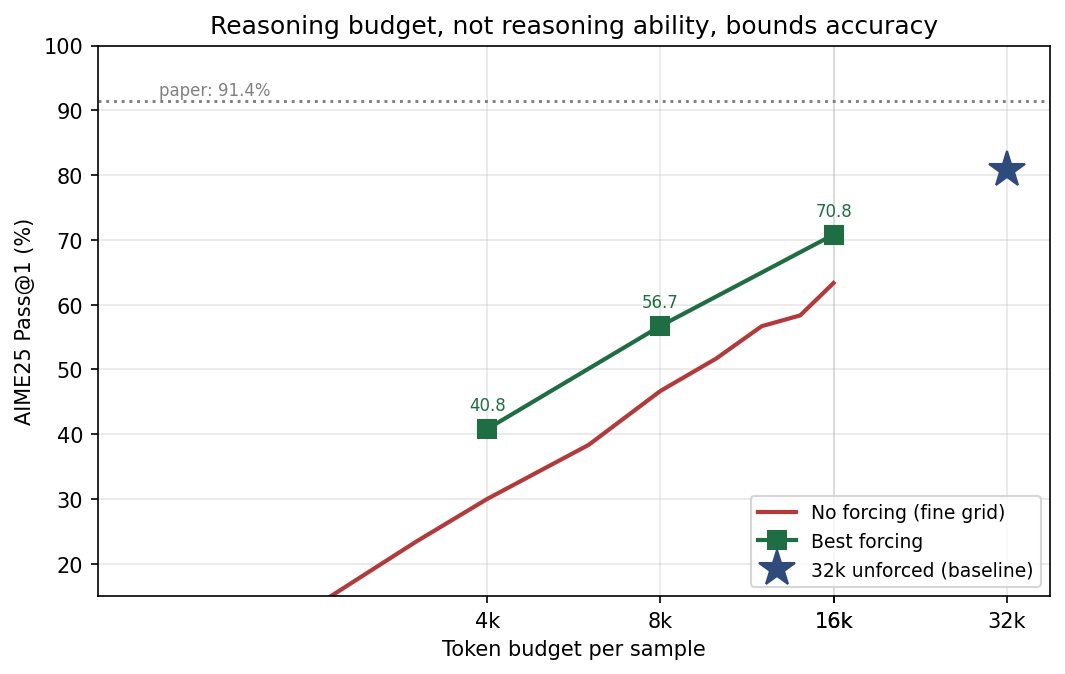
\includegraphics[width=0.85\textwidth]{figures/fig3_main_result.png}
\caption[Accuracy versus generation budget]{Accuracy against generation budget,
with and without budget forcing. The dotted line marks the accuracy reported in
\cite{vibethinker} under an unconstrained budget.}
\label{fig:main}
\end{figure}

\begin{table}[htbp]
\centering
\caption{Accuracy and truncation rate against budget (no forcing)}
\label{tab:curve}
\small
\begin{tabular}{@{}rrr@{\hspace{2.2em}}rrr@{}}
\toprule
\textbf{Budget} & \textbf{Pass@1} & \textbf{Truncated} &
\textbf{Budget} & \textbf{Pass@1} & \textbf{Truncated} \\
\midrule
1K & 3.3\%  & 100.0\% & 8K  & 46.7\% & 67.5\% \\
2K & 13.3\% & 98.3\%  & 10K & 51.7\% & 63.3\% \\
3K & 23.3\% & 92.5\%  & 12K & 56.7\% & 59.2\% \\
4K & 30.0\% & 87.5\%  & 14K & 58.3\% & 53.3\% \\
6K & 38.3\% & 77.5\%  & 16K & 63.3\% & 48.3\% \\
\bottomrule
\end{tabular}
\end{table}

Figure~\ref{fig:trunc} plots truncation rate against accuracy across the same
range. The two curves move in close inverse correspondence, which is the
signature the termination hypothesis predicts.

\begin{figure}[htbp]
\centering
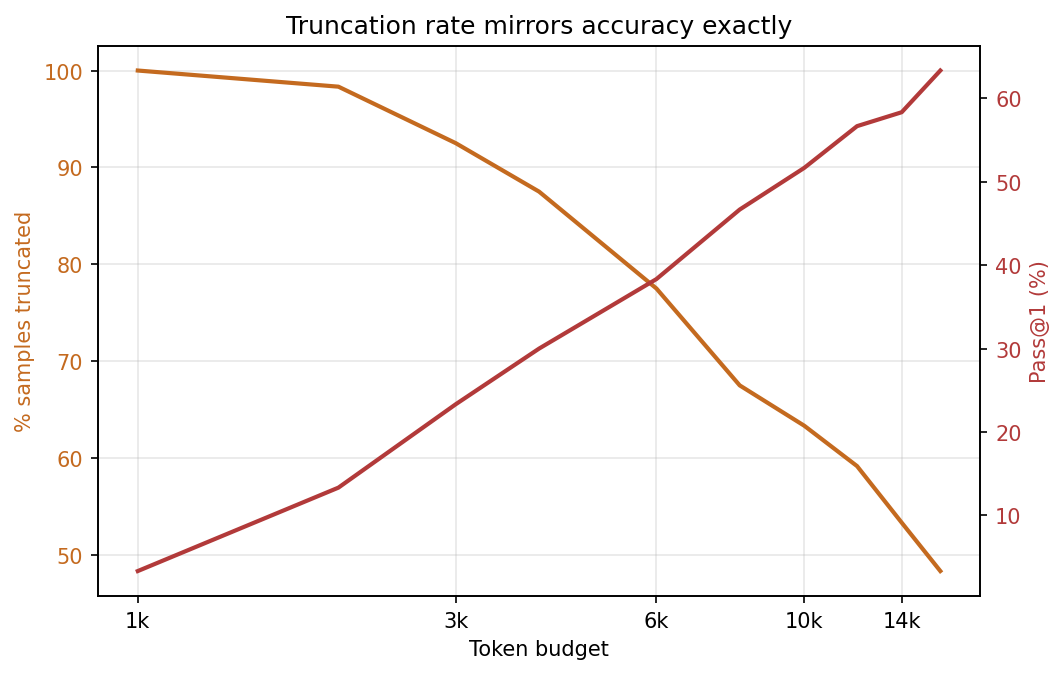
\includegraphics[width=0.85\textwidth]{figures/fig4_truncation.png}
\caption[Truncation rate against accuracy]{Truncation rate and accuracy move
inversely with budget. The left axis gives the percentage of samples cut off by
the budget; the right axis gives Pass@1 over the same samples.}
\label{fig:trunc}
\end{figure}

Table~\ref{tab:curve} also reveals a subtlety. Accuracy exceeds the natural
termination rate by 12 to 18 points at every budget, because the model
sometimes writes an intermediate \boxedans{} expression mid-derivation which the
parser recovers even though the trace never terminated. The unforced baseline
therefore already captures some truncated-but-answered samples, and any
evaluation of forcing must account for this.

Figure~\ref{fig:lengths} shows the reasoning-length distribution. It is strongly
bimodal. Note that the distribution is \emph{right-censored} at 16{,}384 tokens:
the mass at the upper limit reflects the imposed cap, not a natural stopping
point of the model.

\begin{figure}[htbp]
\centering
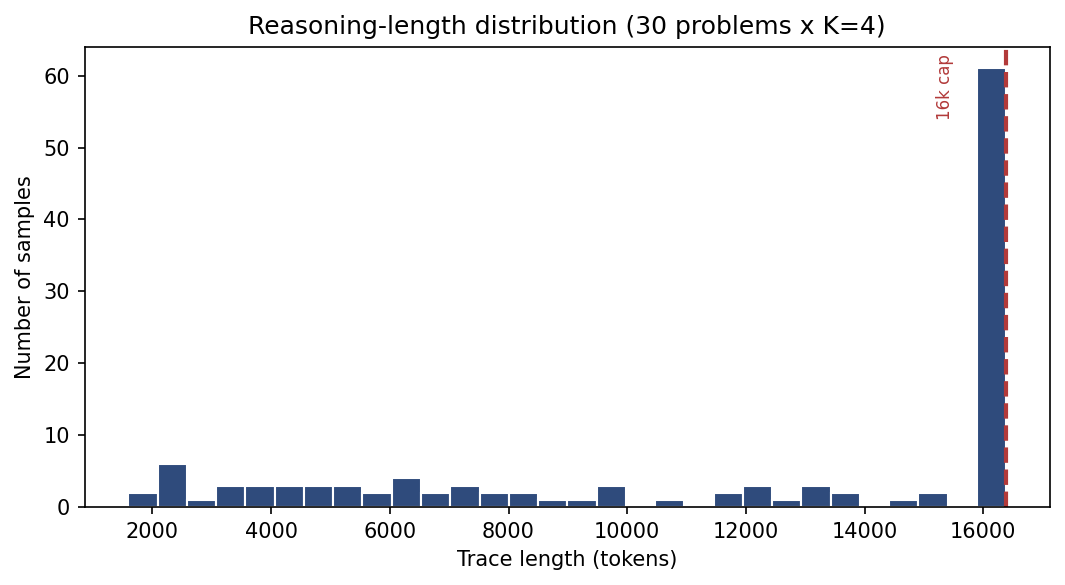
\includegraphics[width=0.85\textwidth]{figures/fig5_lengths.png}
\caption[Reasoning-length distribution]{Distribution of reasoning-trace lengths
over 30 problems $\times$ $K{=}4$ samples. The distribution is right-censored at
16{,}384 tokens; the spike at the cap is an artifact of the imposed limit.}
\label{fig:lengths}
\end{figure}

\section{Effect of Budget Forcing}

Table~\ref{tab:main} presents the principal result.

\begin{table}[htbp]
\centering
\caption{Effect of budget forcing on AIME 2025 Pass@1}
\label{tab:main}
\small
\begin{tabular}{@{}lrrrcc@{}}
\toprule
\textbf{Budget} & \textbf{No forcing} & \textbf{+ Forcing} & \textbf{Gain} &
\textbf{95\% CI} & \textbf{McNemar $p$} \\
\midrule
4K  & 27.5\% / 30.0\% & 40.8\% & $+13.3$ & $[+7.5,+20.0]$ & --- \\
8K  & 46.7\%          & 55.8\% & $+9.1$  & $[+5.0,+15.8]$ & $\mathbf{0.0026}$ \\
16K & 63.3\%          & 70.8\% & $+7.5$  & $[+3.3,+12.5]$ & $\mathbf{0.0077}$ \\
32K & 80.8\%          & not measured & --- & --- & --- \\
\bottomrule
\end{tabular}
\end{table}

The gain is significant at every budget at which the paired test could be
applied. The 4K row lists two baselines because that budget was measured both by
a dedicated generation run (27.5\%) and by trace truncation (30.0\%); the
2.5-point difference corresponds to three samples and lies within sampling
noise.

The magnitude of the gain decreases as the budget grows, from $+13.3$ at 4K to
$+7.5$ at 16K, which follows directly from there being fewer truncated samples
to recover.

\section{Is Budget Forcing Ever Harmful?}

Because forcing overwrites whatever answer a truncated trace already contained,
the aggregate gain could in principle conceal destroyed correct answers. The
paired contingency in Table~\ref{tab:paired} resolves this.

\begin{table}[htbp]
\centering
\caption{Paired contingency for budget forcing (truncated samples only)}
\label{tab:paired}
\small
\begin{tabular}{@{}lrrrrrr@{}}
\toprule
\textbf{Budget} & \textbf{Truncated} & \textbf{$b$ rescued} &
\textbf{$c$ damaged} & \textbf{right$\to$right} & \textbf{$\chi^2$} & \textbf{$p$} \\
\midrule
8K  & 81 & 11 & \textbf{0} & 17 & 9.09 & 0.0026 \\
16K & 58 & 9  & \textbf{0} & 14 & 7.11 & 0.0077 \\
\bottomrule
\end{tabular}
\end{table}

Across 139 interventions, $c = 0$: not one correct answer was converted into an
incorrect one. The \emph{right}$\to$\emph{right} column explains why. Thirty-one
truncated traces already contained a correct \boxedans{} expression; forcing
overwrote every one of them and re-derived the identical correct value. Once the
model has established a result firmly enough to state it once, being compelled
to state it again reproduces it, because the necessary information is present in
the context.

A direct consequence is that a hybrid policy which preserves an existing answer
and forces only when none is present scores identically to unconditional
forcing. The additional logic is therefore unnecessary; the simpler procedure is
already optimal.

\section{Sensitivity to the Forcing Phrase}

Table~\ref{tab:variants} compares three phrasings.

\begin{table}[htbp]
\centering
\caption{Comparison of forcing phrasings}
\label{tab:variants}
\small
\begin{tabular}{@{}lrrr@{\hspace{2em}}rr@{}}
\toprule
& \multicolumn{3}{c}{\textbf{Pass@1}} & \multicolumn{2}{c}{\textbf{Cost (min)}} \\
\cmidrule(lr){2-4}\cmidrule(l){5-6}
\textbf{Budget} & $V_1$ bare & $V_3$ deadline & $V_2$ summarise &
$V_1$ & $V_2$ \\
\midrule
8K  & 55.8\% & 55.8\% & 56.7\% & 21.2 & 47.8 \\
16K & 70.8\% & 70.8\% & 70.8\% & 54.9 & 117.3 \\
\bottomrule
\end{tabular}
\end{table}

At 16K all three are identical. At 8K the two-stage variant leads by 0.9 points,
which is one sample out of 120 and is not a detectable effect. The two-stage
variant nevertheless costs $2.1\times$ more computation at both budgets.

This is a negative result with a clean interpretation. What the intervention
supplies is not a better prompt but \emph{permission to stop}. Elaborating the
request adds cost without adding information, because the information the model
needs is already in its own preceding trace.

It should be noted that the wall-clock cost of forcing is dominated by prefill,
that is, by re-reading the stored trace. The forcing step itself generated only
about five tokens per intervened sample. An implementation that retained the
key-value cache rather than reprocessing the prefix would render forcing very
nearly free; the timings above should not be read as an intrinsic cost of the
method.

\section{Upper Bounds}

\subsection{The selection ceiling}

For any method that selects among $k$ already-generated samples, accuracy is
bounded above by $\text{pass}@k$. Table~\ref{tab:oracle} compares this bound
against forcing.

\begin{table}[htbp]
\centering
\caption{Budget forcing against the selection oracle}
\label{tab:oracle}
\small
\begin{tabular}{@{}lrr@{}}
\toprule
\textbf{Budget} & \textbf{Unforced pass@4 (oracle)} & \textbf{Forced pass@1} \\
\midrule
4K  & 40.0\% & \textbf{40.8\%} \\
8K  & 53.3\% & \textbf{55.8\%} \\
16K & \textbf{73.3\%} & 70.8\% \\
\bottomrule
\end{tabular}
\end{table}

At 4K and 8K a single forced sample outperforms the best of four unforced
samples. Forcing is not bounded by $\text{pass}@k$ because it does not choose
among existing answers; it produces a new one conditioned on partial reasoning.
This quantifies why selection-based test-time methods are ill-suited to this
regime: a \emph{perfect} selector over four samples would reach 53.3\% at 8K,
whereas forcing reaches 55.8\%. At 16K the ordering reverses, consistent with
the mechanism, since more samples terminate naturally and selection has more
genuine answers to arbitrate between.

This comparison places forced $\text{pass}@1$ against unforced
$\text{pass}@4$. Forced $\text{pass}@4$ was not computed, so the comparison is
favourable to forcing in the sense that it grants the oracle four samples and
forcing one.

\subsection{The extraction ceiling}

A recovery rate is meaningless without the maximum recoverable.
Table~\ref{tab:ceiling} restricts attention to the population forcing can act
upon, namely samples that were both truncated and incorrect, and estimates how
many of those contain the correct answer anywhere in their final fifth. A
false-positive control, searching each trace for a \emph{different} problem's
answer, calibrates the spurious match rate.

\begin{table}[htbp]
\centering
\caption{Extraction ceiling on the recoverable population}
\label{tab:ceiling}
\small
\begin{tabular}{@{}lrrrrrrrc@{}}
\toprule
\textbf{Budget} & \textbf{Trunc.} & \textbf{Already ok} & \textbf{Rescuable} &
\textbf{Has ans.} & \textbf{FP} & \textbf{Ceiling} & \textbf{Rescued} &
\textbf{Captured} \\
\midrule
8K  & 81 & 17 & 64 & 16 & 2 & 14 & 11 & 78.6\% \\
16K & 58 & 14 & 44 & 11 & 0 & 11 &  9 & 81.8\% \\
\bottomrule
\end{tabular}
\end{table}

Forcing captures approximately four fifths of the recoverable signal. Wilson
95\% intervals are $[52\%,92\%]$ at 8K and $[52\%,95\%]$ at 16K; the ceiling
population is small, so the point estimates are imprecise, but the lower bounds
lie well above the level at which improved extraction would repay effort. The
false-positive control ran at 0--4.9\% against a signal of 32--41\%, so text
matching is eight to twelve times above noise.

A more consequential observation is visible in the \textbf{Has ans.} column.
Only 16 of 64 rescuable traces at 8K, and 11 of 44 at 16K, mention the correct
answer anywhere in their final fifth. Roughly three quarters of failures never
derived the answer at all, and no extraction procedure could recover them. The
remaining headroom therefore lies in \emph{generating} reasoning, not in reading
it out.

\section{Discussion}

The mechanism by which forcing succeeds and fails is visible directly in the
two-stage variant's intermediate summaries. On problem 1, whose answer is 588,
three of four summaries contain genuine derived quantities, and forcing yields
588. On problem 13, whose answer is 60, the summaries are still establishing the
problem setup, and forcing yields confident but incorrect values of 124 and 184.

The generalisation is that budget forcing recovers answers that are
\emph{already latent} in the trace and cannot manufacture reasoning that has not
occurred. This single statement accounts for all four principal findings: the
gain is real because latent answers are common; the gain is bounded because most
failures are genuinely incomplete; forcing is non-destructive because a latent
answer is stable under re-elicitation; and the phrasing is irrelevant because
what is supplied is permission to conclude rather than any additional
information.

There is a practical consequence for evaluation methodology. Any benchmark that
imposes a generation cap on a long-horizon reasoning model is measuring a
composite of reasoning ability and termination behaviour, and reporting it as
though it were reasoning ability alone. Under such protocols the trivially cheap
intervention studied here is worth 7 to 13 points, which is larger than the
margin separating many published systems.

%=============================================================================
% CHAPTER 5
%=============================================================================
\chapter{Conclusions}

\section{Summary}

This project examined whether the accuracy loss suffered by a compact reasoning
model under a constrained generation budget reflects a failure of reasoning or a
failure of termination. Evaluating VibeThinker-3B on AIME 2025 across budgets
from one thousand to thirty-two thousand tokens, without modifying any weights,
the two failure modes separate cleanly: among samples that terminated naturally
essentially all were correct, whereas truncated samples scored zero not because
their reasoning was wrong but because no answer had been written down.

Budget forcing, a lightweight intervention that compels commitment at the budget
limit, improved accuracy by 7.5 to 13.3 points, significant at every budget by
McNemar's test. Across 139 interventions it never converted a correct answer
into an incorrect one. Three phrasings proved statistically indistinguishable,
and an elaborate two-stage variant cost $2.1\times$ more computation for no
measurable benefit. A single forced sample outperformed the best of four
unforced samples at the smaller budgets, establishing that the method exceeds
the ceiling of any selection-based technique. Restricting to the recoverable
population, forcing captures roughly 80\% of the answers latent in truncated
traces.

The complete study consumed 22.6 GPU-hours on freely available hardware,
demonstrating that a controlled inference-time investigation of a frontier-class
compact model is within reach of an individual student.

\section{Limitations}

The limitations below bound what these results support.

\begin{itemize}
\item \textbf{One model, one benchmark, one seed.} Confidence intervals are
binomial over 120 samples, and no run-to-run variance estimate exists. The
defensible claim is that the effect exceeds plausible sampling noise, not that
it has been replicated.
\item \textbf{Small sample count.} $K = 4$ is adequate for $\text{pass}@1$ but
limits per-problem resolution and widens every interval.
\item \textbf{Small ceiling population.} The extraction-ceiling estimate rests
on 11 to 14 samples, so its 95\% interval spans roughly $[52\%,95\%]$.
\item \textbf{Benchmark substitution.} AIME 2026 was unavailable publicly and
AIME 2025 was used instead. AIME 2025 predates the subject publication and lay
within its evaluation scope; the reproduced accuracy is \emph{below} the
published figure, which argues against contamination, but no independent
decontamination check was performed.
\item \textbf{Context length was not held constant.} The parameter
\texttt{max\_model\_len} differed across arms (10240, 18432, 32768) for memory
reasons. It does not affect sampling logits, and an 8K condition measured under
two different values agreed within noise, but it was not controlled and no claim
that it was is made.
\item \textbf{Cost figures are implementation-bound.} Forcing's wall-clock cost
is prefill arising from reprocessing each stored trace. A cache-reusing
implementation would make it nearly free.
\item \textbf{Two conditions were not measured.} Forcing at 32K was not run; the
observed trend extrapolates to roughly $+5$ points, but this is an extrapolation.
Forced $\text{pass}@4$ was likewise not computed, so the oracle comparison is
not like-for-like.
\item \textbf{A superseded metric.} An earlier ceiling estimate divided rescued
samples by a denominator that proved to coincide with the already-correct set,
making numerator and denominator disjoint. It was retracted and replaced by
Table~\ref{tab:ceiling}. It is recorded here because the error was detected
after the figure had been computed, and transparency about such corrections is
part of the record.
\end{itemize}

\section{Future Improvement}

Four directions follow from the results.

\textbf{Cache-reusing forcing.} Retaining the key-value cache instead of
reprocessing the prefix would reduce the intervention's cost to roughly the five
tokens it actually generates, making it essentially free and suitable for
routine inclusion in evaluation harnesses.

\textbf{Learned termination.} Since roughly three quarters of failures never
derive the answer, the greater opportunity lies in making the model conclude
sooner rather than in extracting more from incomplete traces. A model trained or
prompted to recognise when it has established a result, rather than continuing
to verify, would address the cause rather than the symptom.

\textbf{Generality.} The study covers one model on one benchmark. Whether the
termination-versus-capability decomposition holds for other compact reasoning
models, and on code generation and scientific reasoning as well as mathematics,
is open. The methodology transfers directly, and the prefix-consistency identity
makes such a sweep affordable.

\textbf{Evaluation protocol.} If capped-budget evaluation systematically
conflates reasoning ability with termination behaviour, benchmark reporting
should separate the two. Publishing the truncation rate alongside accuracy would
cost nothing and would make results across differing budgets comparable.

%=============================================================================
% REFERENCES
%=============================================================================
\begin{thebibliography}{99}
\addcontentsline{toc}{chapter}{References}

\bibitem{vibethinker}
S. Xu, S. Liu, W. Wang, J. Min, Y. Dai, Z. Yin, Y. Chen, X. Zhou and J. Zhang,
``VibeThinker-3B: Exploring the frontier of verifiable reasoning in small
language models,'' \emph{arXiv preprint} arXiv:2606.16140, 2026.

\bibitem{s1}
N. Muennighoff, Z. Yang, W. Shi, X. L. Li, L. Fei-Fei, H. Hajishirzi,
L. Zettlemoyer, P. Liang, E. Cand\`{e}s and T. Hashimoto, ``s1: Simple test-time
scaling,'' \emph{arXiv preprint} arXiv:2501.19393, 2025.

\bibitem{deepseekr1}
D. Guo, D. Yang, H. Zhang, J. Song, R. Zhang, R. Xu, Q. Zhu, S. Ma, P. Wang and
X. Bi, ``DeepSeek-R1: Incentivizing reasoning capability in LLMs via
reinforcement learning,'' \emph{arXiv preprint} arXiv:2501.12948, 2025.

\bibitem{deepseekmath}
Z. Shao, P. Wang, Q. Zhu, R. Xu, J. Song, X. Bi, H. Zhang, M. Zhang, Y. K. Li
and Y. Wu, ``DeepSeekMath: Pushing the limits of mathematical reasoning in open
language models,'' \emph{arXiv preprint} arXiv:2402.03300, 2024.

\bibitem{selfconsistency}
X. Wang, J. Wei, D. Schuurmans, Q. Le, E. Chi, S. Narang, A. Chowdhery and
D. Zhou, ``Self-consistency improves chain of thought reasoning in language
models,'' \emph{International Conference on Learning Representations}, 2023.

\bibitem{selfrefine}
A. Madaan, N. Tandon, P. Gupta, S. Hallinan, L. Gao, S. Wiegreffe, U. Alon,
N. Dziri, S. Prabhumoye and Y. Yang, ``Self-Refine: Iterative refinement with
self-feedback,'' \emph{Advances in Neural Information Processing Systems},
vol. 36, pp. 46534--46594, 2023.

\bibitem{qwen25coder}
B. Hui, J. Yang, Z. Cui, J. Yang, D. Liu, L. Zhang, T. Liu, J. Zhang, B. Yu and
K. Dang, ``Qwen2.5-Coder technical report,'' \emph{arXiv preprint}
arXiv:2409.12186, 2024.

\bibitem{vllm}
W. Kwon, Z. Li, S. Zhuang, Y. Sheng, L. Zheng, C. H. Yu, J. Gonzalez, H. Zhang
and I. Stoica, ``Efficient memory management for large language model serving
with PagedAttention,'' \emph{Proceedings of the 29th Symposium on Operating
Systems Principles}, pp. 611--626, 2023.

\bibitem{mcnemar}
Q. McNemar, ``Note on the sampling error of the difference between correlated
proportions or percentages,'' \emph{Psychometrika}, vol. 12, no. 2,
pp. 153--157, 1947.

\bibitem{wilson}
E. B. Wilson, ``Probable inference, the law of succession, and statistical
inference,'' \emph{Journal of the American Statistical Association}, vol. 22,
no. 158, pp. 209--212, 1927.

\bibitem{repo}
A. Ahmad, ``llm-budget-forcing: Code and data for this project.'' Accessed on:
Aug.\ 2026. [Online]. Available:
\url{https://github.com/abuahmad369/llm-budget-forcing}

\end{thebibliography}

\end{document}
